\chapter{光錐、測地線與史瓦西視界}

視界問題始於狹義相對論中已有的一項區分：兩個鄰近事件之間的分離，可以是類時、類空或類光。曲率並不會取消這種分類；它使光錐成為局部的物件，在每個事件處各不相同，也使度規本身具有動力學。一旦度規已知，自由下落粒子的運動便遵循固有時原理，與描述平直時空中自由相對論粒子的原理相同。

我們會兩度運用這項原理。首先，它必須在弱場下重現牛頓運動；接著，我們會將它應用於史瓦西度規。在那裡，時間、徑向距離與速度的意義會變得出乎意料地微妙。

\section{類時、類空與類光間隔}

在平直時空中，取\(c=1\)，固有時微元為
\begin{equation}
d\tau^2=dt^2-dx^2-dy^2-dz^2.
\label{eq:l5-minkowski-proper-time}
\end{equation}
在非相對論近似下，恢復\(c\)很有用：
\begin{equation}
d\tau^2
=dt^2-\frac{dx^2+dy^2+dz^2}{c^2}.
\label{eq:l5-minkowski-c}
\end{equation}
記號\(d\tau^2\)不保證右側為正。它的符號可用來分類位移：
\begin{align}
d\tau^2>0
&\quad\Longleftrightarrow\quad \text{time-like},\\
d\tau^2=0
&\quad\Longleftrightarrow\quad \text{light-like},\\
d\tau^2<0
&\quad\Longleftrightarrow\quad \text{space-like}.
\end{align}
對類空位移，方便的做法是定義正的固有距離
\begin{equation}
ds^2=-d\tau^2
=dx^2+dy^2+dz^2-dt^2
\qquad(c=1).
\label{eq:l5-proper-distance}
\end{equation}

光錐將這三種可能性組織起來。類光方向位於光錐表面，而非錐內；類時方向位於錐內，類空方向則位於錐外。上半部與下半部分別代表未來光錐和過去光錐。

\begin{figure}[htbp]
\centering
\includegraphics[width=0.82\textwidth]{lecture_05_figure_02.png}
\caption{黑板上呈現的固有時、固有距離與因果錐。光線位於錐面上；錐內為類時，錐外為類空。}
\lectureframe{00:05:44}
\end{figure}

\begin{figure}[htbp]
\centering
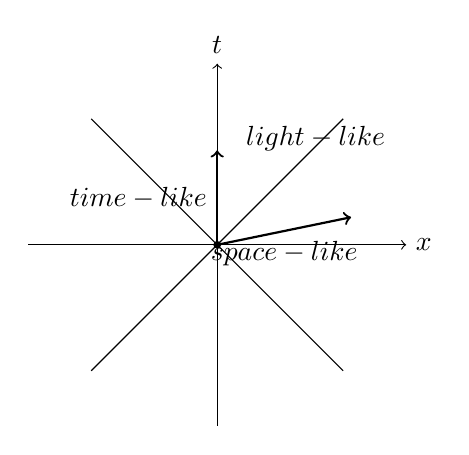
\begin{tikzpicture}[scale=1.0]
\draw[->] (0,-2.3) -- (0,2.3) node[above] {\(t\)};
\draw[->] (-2.4,0) -- (2.4,0) node[right] {\(x\)};
\draw (-1.6,1.6) -- (0,0) -- (1.6,1.6);
\draw (-1.6,-1.6) -- (0,0) -- (1.6,-1.6);
\fill (0,0) circle (1.4pt);
\draw[->,thick] (0,0) -- (0,1.2)
  node[midway,left] {\(\text{time-like}\)};
\draw[->,thick] (0,0) -- (1.7,0.35)
  node[midway,below] {\(\text{space-like}\)};
\node at (1.25,1.35) {\(\text{light-like}\)};
\end{tikzpicture}
\caption{二維時空截面中的因果分類。}
\end{figure}

這些間隔具有操作上的意義。固有時是沿類時世界線攜帶的時鐘所顯示的時間；固有距離則是適當配置的一組量尺，在類空分離的事件之間測得的距離。它們不只是二次型中正負號的名稱。

\section{洛倫茲號差與每個事件處的光錐}

採用正號較多的張量約定時，平直度規的分量為
\begin{equation}
\eta_{\mu\nu}=\operatorname{diag}(-1,1,1,1),
\label{eq:l5-eta}
\end{equation}
而
\begin{equation}
d\tau^2=-\eta_{\mu\nu}\,dx^\mu dx^\nu.
\label{eq:l5-proper-time-eta}
\end{equation}
所示矩陣是二階張量在一個特別簡單的基底中的表示。它的不變特徵是號差：一個負方向與三個正方向，
\begin{equation}
\operatorname{signature}(\eta)=(-,+,+,+).
\label{eq:l5-lorentz-signature}
\end{equation}
有兩個負號的度規會有兩個時間方向。這類號差可在數學上研究，但並不描述此處所假設的時空。

在彎曲時空中，度規分量會隨位置改變：
\begin{equation}
g_{\mu\nu}=g_{\mu\nu}(x).
\label{eq:l5-position-metric}
\end{equation}
但每個事件處的度規仍須具有洛倫茲號差。因此，每個事件都有自己的類時方向、類光邊界與類空方向。座標圖中的光錐可能隨位置傾斜或壓扁，但因果分類仍然成立。

\begin{figure}[htbp]
\centering
\includegraphics[width=0.86\textwidth]{lecture_05_figure_03.png}
\caption{位置相關的度規\(g_{\mu\nu}(x)\)、因果分類標記，以及局部光錐示意圖。}
\lectureframe{00:09:41}
\end{figure}

\begin{figure}[htbp]
\centering
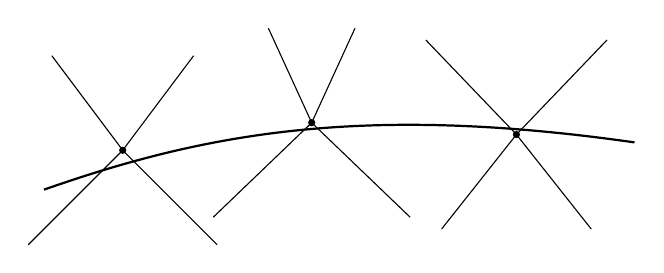
\begin{tikzpicture}[scale=1.0]
\draw[thick] (-4,-0.5) .. controls (-2,0.2) and (0,0.6) .. (3.5,0.1);
\foreach \x/\y/\a/\b in {-3/0/0.9/1.2, -0.6/0.35/0.55/1.25,
                          2.0/0.2/1.15/0.95} {
  \fill (\x,\y) circle (1.3pt);
  \draw (\x,\y) -- ++(-\a,1.2);
  \draw (\x,\y) -- ++(\a,1.2);
  \draw (\x,\y) -- ++(-\b,-1.2);
  \draw (\x,\y) -- ++(\b,-1.2);
}
\end{tikzpicture}
\caption{相鄰的局部光錐。座標圖中的形狀可以改變，但哪些向量屬於類時、類光或類空仍不變。}
\end{figure}

\begin{classroomqa}
\audiencequestion{唯一的負特徵值是否選定了唯一的時間方向？}
\lecturerresponse{使所示矩陣對角化的基底有一個負號的基底方向，但這並未選出優先的觀測者，也未選定唯一的物理箭頭。洛倫茲變換會混合時間座標與空間座標，而光錐內的每個向量都是類時的。不變的對象是光錐及一負三正的號差，而不是某個特殊的類時向量。
\lecturetimestamp{00:12:17--00:17:24}}
\end{classroomqa}

\begin{classroomqa}
\audiencequestion{為什麼局部光錐的兩幅圖會有不同形狀？}
\lecturerresponse{座標會改變圖上的形狀。例如，將\(x\)換成經過重新縮放的座標，會改變光線斜率的數值，因此光錐看起來會變窄或變寬。更一般的座標變換還可能使光錐傾斜。兩幅圖表示的是同一事件與相同的因果關係。在彎曲時空中，不同事件處的光錐也屬於不同的切空間，因此若要比較它們，就需要度規與輸運規則。
\lecturetimestamp{00:13:37--00:15:59}}
\end{classroomqa}

\section{以變分問題表述測地線}

自由運動的粒子沿著時空測地線運動。使用仿射參數\(\lambda\)時，其微分形式為
\begin{equation}
\frac{d^2x^\mu}{d\lambda^2}
+\Gamma^\mu{}_{\rho\sigma}
\frac{dx^\rho}{d\lambda}
\frac{dx^\sigma}{d\lambda}=0.
\label{eq:l5-geodesic}
\end{equation}
聯絡描述粒子運動時，切向量如何保持與自身平行。

另一種表述通常更便於計算。在度規為\(g_{mn}\)的黎曼空間中，曲線長度為
\begin{equation}
s=\int ds
=\int\sqrt{g_{mn}\,dx^m dx^n}.
\label{eq:l5-spatial-length}
\end{equation}
當路徑在端點固定的條件下作微小變動時，測地線使這個長度取駐值。此積分就是沿曲線累加無窮小長度；相應的歐拉--拉格朗日方程是一個二階微分方程，形式上類似力學中的運動方程。

對類時世界線而言，空間長度由固有時取代：
\begin{equation}
\tau
=\int\sqrt{-g_{\mu\nu}\,dx^\mu dx^\nu}.
\label{eq:l5-proper-time-functional}
\end{equation}
類時測地線使\(\tau\)取駐值；在共軛點出現之前，它對鄰近的自由下落路徑而言，局部取最大值。乘上\(-m\)便得到粒子作用量
\begin{equation}
A=-m\tau
=-m\int\sqrt{-g_{\mu\nu}\,dx^\mu dx^\nu}.
\label{eq:l5-particle-action}
\end{equation}
因此，同一條路徑使\(A=-m\tau\)局部取最小值。固有時取駐值與所選作用量的符號不同，這便消除了表面上最大值與最小值之間的歧義。

\section{從固有時到一般拉格朗日量}

\eqref{eq:l5-particle-action}中的作用量具有幾何意義，但也可以改寫成力學中熟悉的形式。以座標\(t\)為世界線的參數，將各微分除以\(dt\)，再把剩下的\(dt\)因子移到積分號外的平方根：
\begin{align}
A
&=-m\int\sqrt{-g_{\mu\nu}(x)\,dx^\mu dx^\nu}\\
&=-m\int
\sqrt{-g_{\mu\nu}(x)
\frac{dx^\mu}{dt}\frac{dx^\nu}{dt}}\,dt.
\label{eq:l5-action-t}
\end{align}
時間分量滿足\(dt/dt=1\)；空間分量則是一般的座標速度。因此可寫成
\begin{equation}
\begin{aligned}
A&=\int L\,dt,\\
L&=-m\sqrt{-g_{\mu\nu}(x)\dot x^\mu\dot x^\nu},\\
\dot x^\mu&=\frac{dx^\mu}{dt}.
\end{aligned}
\label{eq:l5-relativistic-lagrangian}
\end{equation}

\begin{figure}[htbp]
\centering
\includegraphics[width=0.88\textwidth]{lecture_05_figure_05.png}
\caption{將世界線作用量改寫為慣用形式\(A=\int L\,dt\)。}
\lectureframe{00:27:00}
\end{figure}

\begin{figure}[htbp]
\centering
\includegraphics[width=0.88\textwidth]{lecture_05_figure_06.png}
\caption{稍後的黑板畫面，已將相對論性拉格朗日量單獨列出。}
\lectureframe{00:28:59}
\end{figure}

\begin{classroomqa}
\audiencequestion{這個作用量中的時空指標應該用希臘字母嗎？}
\lecturerresponse{是的。希臘指標涵蓋時間與所有空間座標；若有助於區分，拉丁指標可以專指空間座標。
\lecturetimestamp{00:25:53--00:26:03}}
\end{classroomqa}

\begin{classroomqa}
\audiencequestion{為什麼這個平方根表示式稱為拉格朗日量？}
\lecturerresponse{將作用量寫成\(A=\int L\,dt\)後，被積函數就是拉格朗日量。這不只是定義：對該被積函數取變分，會得到歐拉--拉格朗日方程
\[
\frac{d}{dt}
\left(\frac{\partial L}{\partial\dot x^\mu}\right)
=\frac{\partial L}{\partial x^\mu},
\]
只要一致地處理參數化，這些方程便等價於測地線方程。
\lecturetimestamp{00:28:36--00:29:02}}
\end{classroomqa}

對有質量粒子而言，世界線是類時的，因此平方根內的量為正。類空路徑描述的是超光速運動，不是一般有質量粒子的軌跡。給定度規後，可以計算克里斯托費爾符號並使用\eqref{eq:l5-geodesic}來求出粒子的路徑，也可以對\eqref{eq:l5-relativistic-lagrangian}套用歐拉--拉格朗日方程。證明兩種方法等價是一項有用的練習；通常由作用量出發的推導較短。

\section{牛頓極限}

考慮球形源外部的弱靜態引力場。從平直時空出發，讓\(dt^2\)的係數略微偏離一：
\begin{equation}
d\tau^2
=\left(1+\frac{2u(\mathbf{x})}{c^2}\right)dt^2
-\frac{d\mathbf{x}^2}{c^2},
\label{eq:l5-weak-metric}
\end{equation}
其中\(u\)將作為牛頓位勢。這個假設必須經過檢驗，不能只憑命名便視為成立。

有量綱的粒子作用量為
\begin{equation}
A=-mc^2\int
\sqrt{1+\frac{2u}{c^2}
-\frac{\dot{\mathbf{x}}^{\,2}}{c^2}}\,dt.
\label{eq:l5-weak-action}
\end{equation}
\(u/c^2\)與\(\dot{\mathbf{x}}^{\,2}/c^2\)都很小。保留它們的一階貢獻，
\begin{equation}
\sqrt{1+\epsilon}
=1+\frac{\epsilon}{2}+O(\epsilon^2),
\qquad
\epsilon=\frac{2u-\dot{\mathbf{x}}^{\,2}}{c^2},
\end{equation}
可得
\begin{align}
L
&=-mc^2
\sqrt{1+\frac{2u-\dot{\mathbf{x}}^{\,2}}{c^2}}\\
&=-mc^2-mu+\frac{m}{2}\dot{\mathbf{x}}^{\,2}\\
&\quad+O\!\left(c^{-2}
 [u^2+u\dot{\mathbf{x}}^{\,2}+\dot{\mathbf{x}}^{\,4}]\right).
\label{eq:l5-newton-expansion}
\end{align}
常數的靜止能量項不影響運動方程。剩下的部分為
\begin{equation}
L_{\mathrm{nr}}
=\frac{m}{2}\dot{\mathbf{x}}^{\,2}-m u(\mathbf{x}),
\label{eq:l5-newton-lagrangian}
\end{equation}
因此
\begin{equation}
m\ddot{\mathbf{x}}=-m\boldsymbol{\nabla}u.
\label{eq:l5-newton-equation}
\end{equation}
試驗質量會消去，這正是普遍自由落體所要求的。位能為\(m u\)，而加速度與\(m\)無關。

因此，我們得到弱場下的領先階關係
\begin{equation}
g_{00}=1+\frac{2u}{c^2}+O(c^{-4}).
\label{eq:l5-g00-newton}
\end{equation}
在球形質量\(M\)外部，
\begin{equation}
u(r)=-\frac{GM}{r},
\qquad
g_{00}=1-\frac{2GM}{rc^2}+O(c^{-4}).
\label{eq:l5-g00-spherical}
\end{equation}
這決定了時間分量的一階修正，但尚未決定完整的強場度規。

\section{球座標與第一個史瓦西猜測}

對中心源而言，球座標很自然。本講從赤道面而非極點量起\(\theta\)，因此角向線元素為
\begin{equation}
d\Omega^2=d\theta^2+\cos^2\theta\,d\phi^2.
\label{eq:l5-angular-metric}
\end{equation}
依照這項約定，
\begin{equation}
d\mathbf{x}^2=dr^2+r^2d\Omega^2.
\label{eq:l5-flat-spherical}
\end{equation}
物理結果不受這個類似緯度的\(\theta\)選法影響；若改用較常見的極角，\(\cos^2\theta\)便會換成\(\sin^2\theta\)。

將牛頓時間係數代入，同時讓空間度規保持平直，得到第一個猜測：
\begin{equation}
\begin{aligned}
d\tau^2
&=\left(1-\frac{r_s}{r}\right)dt^2
-\frac{1}{c^2}\left(dr^2+r^2d\Omega^2\right),\\
r_s&=\frac{2GM}{c^2}.
\end{aligned}
\label{eq:l5-naive-schwarzschild}
\end{equation}
這不可能是精確解。當\(r<r_s\)時，\(dt^2\)的係數會改變符號，但所有空間係數仍為負；度規便會失去一個時間方向、三個空間方向的號差。

真空場方程給出所需的徑向係數：
\begin{equation}
\boxed{
d\tau^2
=\left(1-\frac{r_s}{r}\right)dt^2
-\frac{dr^2}{c^2\left(1-r_s/r\right)}
-\frac{r^2}{c^2}d\Omega^2.
}
\label{eq:l5-schwarzschild}
\end{equation}
這就是外部史瓦西度規。當\(r\)穿越\(r_s\)時，\(t\)與\(r\)的係數會同時改變符號，因此洛倫茲號差得以維持。在史瓦西座標中，視界內的徑向座標成為類時，而座標\(t\)成為類空。這種交換表示座標系統在視界處失效，不代表時空幾何本身在局部失效。

\begin{classroomqa}
\audiencequestion{物體下落穿越視界需要多久？}
\lecturerresponse{以遠方觀測者所用的史瓦西座標時間\(t\)來量度，穿越所需時間會延伸至無限；以落體時鐘量得的固有時來看，穿越則在有限時間內發生。兩種時鐘的差異正是視界問題的核心。
\lecturetimestamp{00:54:45--00:55:35}}
\end{classroomqa}

\begin{classroomqa}
\audiencequestion{為什麼要改變徑向係數，而不改變度規的其他部分？}
\lecturerresponse{度規必須維持洛倫茲號差；球對稱性使徑向與角向球面有所區別；而真空場方程會精確決定倒數因子。號差只能提示我們該從何處著手，精確結果則由愛因斯坦方程給出。
\lecturetimestamp{00:55:35--00:56:01}}
\end{classroomqa}

對地球而言，\(r_s\)只有約一公分，位於地球物質內部深處。外部真空度規在此處並不適用，因此地球沒有史瓦西視界。物質內部必須改用內部解，並在表面與外部解銜接。

\begin{classroomqa}
\audiencequestion{如果\(t\)和\(r\)交換座標角色，一般時鐘會怎麼樣？}
\lecturerresponse{時鐘仍會沿類時世界線量度固有時；它不會察覺所選座標已變得不便使用。使用規則的自由落體座標系，可以看到平滑的局部幾何，以及光線穿越視界時的正常局部傳播。
\lecturetimestamp{00:56:35--00:57:50}}
\end{classroomqa}

\subsection{為什麼徑向修正沒有出現在牛頓方程中}

精確度規在位勢的一階就已改變徑向係數：
\begin{equation}
\frac{1}{1-r_s/r}
=1+\frac{r_s}{r}
+O\!\left(\frac{r_s^2}{r^2}\right)
=1-\frac{2u}{c^2}+O(c^{-4}).
\label{eq:l5-radial-expansion}
\end{equation}
為什麼在推導牛頓方程時可以忽略這項改變？在粒子作用量中，它乘上\(\dot r^2/c^2\)。因此，它帶來的第一項修正正比於
\begin{equation}
\frac{u\,\dot r^2}{c^4},
\end{equation}
這超出了\eqref{eq:l5-newton-expansion}保留的階數。對慢速運動的牛頓近似而言，徑向修正可以忽略；但在相對論性運動與視界附近，它就至關重要。這提醒我們：對某種近似而言太小的項，在另一種近似中可能主導所關注的現象。

\section{史瓦西時間中的徑向下落}

令\(c=1\)，先研究徑向運動。圓軌道也很重要，但需納入角向項，因此留待稍後討論。與其說徑向運動是繞行軌道，不如說是直接朝源墜落；而且只需較少代數運算，就能看出視界附近的行為。

\begin{classroomqa}
\audiencequestion{徑向速度中的時間是誰的時間？}
\lecturerresponse{變數上方的點表示對史瓦西座標時間\(t\)微分；這個時間以遠方靜止觀測者的時間為基準。落體觀測者的腕錶量度的是固有時\(\tau\)。若混淆兩者，就會把座標上的敘述誤當成錯誤的局部敘述。
\lecturetimestamp{01:04:03--01:04:47}}
\end{classroomqa}

取\(d\Omega=0\)，並定義
\begin{equation}
a(r)=1-\frac{r_s}{r}.
\label{eq:l5-a-def}
\end{equation}
徑向度規與拉格朗日量為
\begin{align}
d\tau^2&=a\,dt^2-\frac{dr^2}{a},\\
L&=-m\sqrt{a-\frac{\dot r^2}{a}},
\qquad
\dot r=\frac{dr}{dt}.
\label{eq:l5-radial-lagrangian}
\end{align}
由於\(L\)不顯含\(t\)，其哈密頓量守恆。徑向動量為
\begin{equation}
p_r=\frac{\partial L}{\partial\dot r}
=\frac{m\dot r}{a\sqrt{a-\dot r^2/a}},
\label{eq:l5-radial-momentum}
\end{equation}
而
\begin{align}
H
&=p_r\dot r-L\\
&=\frac{ma}{\sqrt{a-\dot r^2/a}}
=E.
\label{eq:l5-radial-energy}
\end{align}
解出座標速度可得
\begin{equation}
\boxed{
\dot r^2
=a^2\left(1-\frac{m^2}{E^2}a\right).
}
\label{eq:l5-radial-velocity}
\end{equation}
黑板上的推導檢查了幾種中間代數形式；方框中的式子才是前後一致的結果。

當\(r\)趨近\(r_s\)時，\(a(r)\)趨近於零，而括號內的因子趨近於一。因此，對入射粒子而言，
\begin{equation}
\frac{dr}{dt}
\sim -\left(1-\frac{r_s}{r}\right)
\longrightarrow 0
\qquad(r\longrightarrow r_s^+)
\label{eq:l5-infall-freeze}
\end{equation}
以史瓦西時間描述時，粒子看起來會減速，並凍結在視界外側。

\begin{classroomqa}
\audiencequestion{\(dr/dt\)的數值減小，是否表示引力變成了斥力？}
\lecturerresponse{不是。粒子在局部並未受到向外的推力。座標\(t\)越來越不適合描述穿越視界的過程，因此每單位\(t\)的徑向位移趨近於零。自由下落世界線上的固有加速度仍為零，而且物體會在有限固有時內到達視界。
\lecturetimestamp{01:14:18--01:16:38}}
\end{classroomqa}

事實上，在視界附近
\begin{equation}
\frac{dt}{dr}
\sim-\frac{1}{1-r_s/r}
=-\frac{r}{r-r_s}.
\end{equation}
其積分會呈對數發散。這證明史瓦西時間趨於無限，卻不表示落體時鐘上的讀數也會無限增大。

\section{徑向光線}

對光而言，同一計算可以用最簡短的方式完成。對徑向零測地線，
\begin{equation}
d\tau^2
=a\,dt^2-\frac{dr^2}{a}=0.
\end{equation}
因此
\begin{equation}
\boxed{
\frac{dr}{dt}
=\pm a(r)
=\pm\left(1-\frac{r_s}{r}\right).
}
\label{eq:l5-radial-light}
\end{equation}
正號表示出射光線，負號表示入射光線。兩者的座標速度在視界處都趨近於零。

\begin{classroomqa}
\audiencequestion{遠離光源時，這個公式給出什麼速度？}
\lecturerresponse{當\(r\)趨近無窮大時，\(a(r)\)趨近於一，因此\(dr/dt\)趨近於\(\pm1\)；恢復單位後則為\(\pm c\)。
\lecturetimestamp{01:21:01--01:21:29}}
\end{classroomqa}

廣義相對論常是如此：原理只需幾行就能說明，座標與計算卻可能變得複雜。方程\eqref{eq:l5-radial-light}很簡單，但要理解它在\(r_s\)附近趨近於零，則須格外小心。這裡談的是座標速度，不是局部慣性觀測者測得的速度。

\section{遠方觀測者所見}

\begin{classroomqa}
\audiencequestion{視界附近發出的光能逃逸嗎？這就是霍金輻射嗎？}
\lecturerresponse{在視界外側不遠處發出的經典出射光線可以向外傳播，但它的史瓦西座標速度起初極小，訊號到達無窮遠時也已大幅延遲並紅移。沿視界發出的光線在這些座標中仍留在視界上；從視界內發出的光線則無法逃出。霍金輻射是與外部幾何相關的量子場效應，不是從內部爬出來的經典光線；本節的計算也沒有推導出霍金輻射。
\lecturetimestamp{01:22:08--01:24:28}}
\end{classroomqa}

\begin{classroomqa}
\audiencequestion{如果光子看起來幾乎靜止，是否就開始顯得有質量？}
\lecturerresponse{不會。自由落體的局部觀測者測得光子始終以\(c\)運動。趨近於零的只有座標比值\(dr/dt\)。不良的座標系不會改變質量、零性質，也不會改變局部測得的光速。
\lecturetimestamp{01:24:31--01:25:26}}
\end{classroomqa}

此處使用的史瓦西形式是真空外部解。恆星、行星或坍縮雲的內部度規不同，必須與外部解銜接。若物質表面位於\(r_s\)之外——如地球遠在其外——外部座標視界就落在真空公式無法延伸穿過物質的範圍之外。若天體坍縮至史瓦西半徑以內，視界便成為物理時空的一部分。

\begin{classroomqa}
\audiencequestion{如果外部觀測者永遠看不到物質穿越視界，黑洞又如何形成或增長？}
\lecturerresponse{這個問題的前提，是把史瓦西時間當成視界處的全域物理時鐘。由此推論黑洞永遠無法增長，聽來似乎合理，實際上卻是錯的。完整回答需要使用能平順穿越視界的座標，並考慮坍縮的全域因果幾何；這項解答留待課程下一階段再談。
\lecturetimestamp{01:27:57--01:29:36}}
\end{classroomqa}

\begin{classroomqa}
\audiencequestion{雷達測速槍會如何測量一輛朝視界下落的汽車？}
\lecturerresponse{汽車下落時，座標速度先增加，之後轉而減小並趨近於零。較晚發出的雷達脈衝仍能在視界外追上汽車，但訊號往返所需時間會愈來愈長。返回訊號的紅移愈來愈大，汽車的影像在\(r_s\)附近看起來會愈來愈慢，並逐漸壓縮。這無法如實呈現駕駛員的局部經驗；駕駛員會在有限固有時內穿越視界。
\lecturetimestamp{01:29:39--01:32:14}}
\end{classroomqa}

\begin{classroomqa}
\audiencequestion{光速只有在狹義相對論中才是常數嗎？}
\lecturerresponse{在廣義相對論中，光速在每個局部慣性系中同樣是常數。與局部時鐘和量尺一同下落的觀測者，測得附近光子的速度為\(c\)。諸如\(dr/dt\)這類座標速度可能改變，因為\(r\)與\(t\)並非整個時空中同一個局部慣性實驗室的讀數。
\lecturetimestamp{01:32:20--01:34:20}}
\end{classroomqa}

\section{史瓦西計算之外的問題}

\begin{classroomqa}
\audiencequestion{統一引力與其他作用力可能是什麼意思？}
\lecturerresponse{一種幾何上的可能性，是以額外的緊緻方向擴充時空。如此一來，高維度規的分量在四維中可以呈現為規範場與純量場，而沿額外方向的動量則可以呈現為電荷。這是與卡魯扎--克萊因構想相關的結構性線索，並非本講已完成的統一理論。
\lecturetimestamp{01:34:22--01:36:08}}
\end{classroomqa}

\begin{classroomqa}
\audiencequestion{不同區域或宇宙的度規號差可以不同嗎？}
\lecturerresponse{經典廣義相對論通常採用固定且非退化的洛倫茲號差。若要改變號差，度規就必須經過退化構形，而標準的經典描述在此處會失效。量子引力或許需要更廣泛的描述方式，但目前尚無公認理論能預測物理上發生號差改變的區域。
\lecturetimestamp{01:36:08--01:38:08}}
\end{classroomqa}

\begin{classroomqa}
\audiencequestion{史瓦西在第一次世界大戰期間服役時，如何找到這個解？}
\lecturerresponse{課堂上強調的這一點，既關乎歷史，也關乎人的處境：史瓦西是一位天文學家，也是一位造詣深厚的數學家。在戰時服役期間，研究愛因斯坦的新方程為他提供了心智上的寄託。
\lecturetimestamp{01:38:11--01:39:02}}
\end{classroomqa}

核心教訓已足夠清楚，可以繼續往下探討。度規同時決定因果錐與自由運動。弱場下的時間分量包含牛頓位勢；精確的史瓦西形式則在\(r=r_s\)處給出座標視界。以史瓦西時間描述，穿越所需時間延伸至無限；但對落體觀測者而言，固有時並非如此。下一個問題是如何從全域角度化解這項反差，以及黑洞如何在遠方影像看似凍結的情況下形成。